% AI-assisted code: generated and revised with Claude Opus 5.5
% under the author's direction; reviewed and tested by the author
% (see the thesis section "Use of AI tools").
% UML object diagram: a snapshot of the committed generation 8 of the recorded
% run runs/eval1_orchestrator_dynamic_bfs_s1 (generation_0008.json, config.yaml).
\documentclass[border=4pt]{standalone}
% Shared TikZ style for the thesis UML figures (standalone documents).
\usepackage[T1]{fontenc}
\usepackage{lmodern}
\usepackage{tikz}
\usetikzlibrary{positioning,arrows.meta,shapes.multipart,shapes.geometric,fit,backgrounds,calc,matrix}
\definecolor{umlfill}{HTML}{F4F6FA}
\definecolor{umlline}{HTML}{3A4150}
\definecolor{umlaccent}{HTML}{0071E3}
\tikzset{
  every node/.style={font=\sffamily\small},
  % class box: \node[class] {Name \nodepart{second} attrs \nodepart{third} ops};
  class/.style={rectangle split, rectangle split parts=3, draw=umlline, fill=umlfill,
    align=left, rectangle split part align={center,left,left}, inner sep=3pt, font=\sffamily\scriptsize},
  % generalisation (hollow triangle), realisation (dashed, hollow triangle)
  inherit/.style={-{Triangle[open,length=7pt,width=7pt]}, draw=umlline},
  realize/.style={-{Triangle[open,length=7pt,width=7pt]}, dashed, draw=umlline},
  % composition (filled diamond at the whole), aggregation (hollow), association, dependency
  compose/.style={{Diamond[length=9pt,width=6pt]}-, draw=umlline},
  aggregate/.style={{Diamond[open,length=9pt,width=6pt]}-, draw=umlline},
  assoc/.style={-, draw=umlline},
  navassoc/.style={-{Straight Barb[length=5pt]}, draw=umlline},
  depend/.style={-{Straight Barb[length=5pt]}, dashed, draw=umlline},
  mult/.style={font=\sffamily\tiny, inner sep=1pt},
  stereo/.style={font=\sffamily\tiny\itshape},
}

\begin{document}
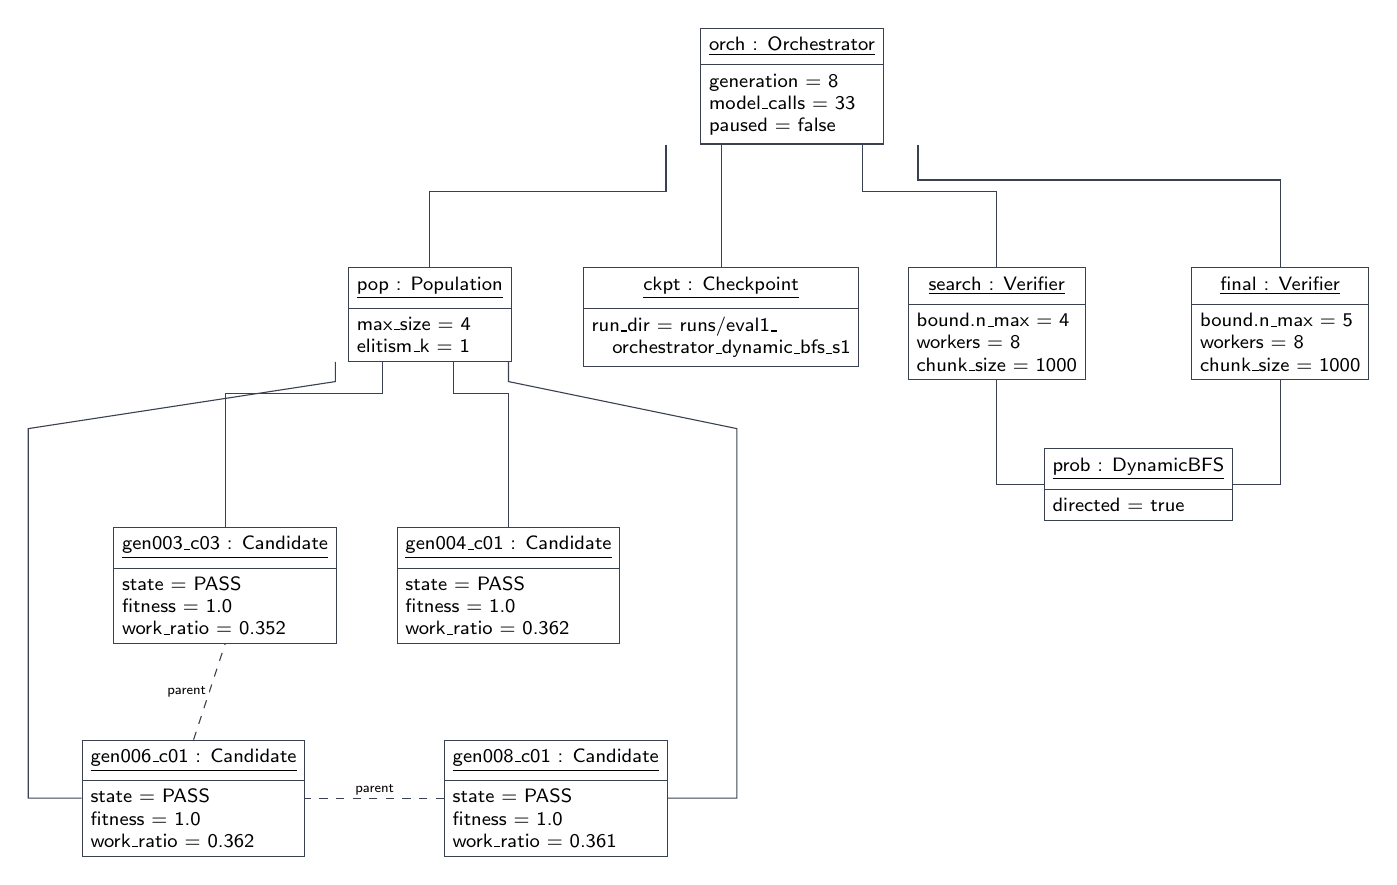
\begin{tikzpicture}[
    obj/.style={rectangle split, rectangle split parts=2, draw=umlline, fill=white,
      align=left, rectangle split part align={center,left}, inner sep=3pt,
      font=\sffamily\scriptsize},
    link/.style={draw=umlline},
    lbl/.style={font=\sffamily\tiny, inner sep=1pt, fill=white}]
  % engine objects
  \node[obj] (orch) at (0,0) {\underline{orch : Orchestrator}
    \nodepart{second} generation = 8\\ model\_calls = 33\\ paused = false};
  \node[obj, anchor=north] (pop) at (-4.6,-2.3) {\underline{pop : Population}
    \nodepart{second} max\_size = 4\\ elitism\_k = 1};
  \node[obj, anchor=north] (sv) at (2.6,-2.3) {\underline{search : Verifier}
    \nodepart{second} bound.n\_max = 4\\ workers = 8\\ chunk\_size = 1000};
  \node[obj, anchor=north] (fv) at (6.2,-2.3) {\underline{final : Verifier}
    \nodepart{second} bound.n\_max = 5\\ workers = 8\\ chunk\_size = 1000};
  \node[obj, anchor=north] (ck) at (-0.9,-2.3) {\underline{ckpt : Checkpoint}
    \nodepart{second} run\_dir = runs/eval1\_\\ \quad orchestrator\_dynamic\_bfs\_s1};
  \node[obj, anchor=north] (pd) at (4.4,-4.6) {\underline{prob : DynamicBFS}
    \nodepart{second} directed = true};
  % the four surviving candidates, oldest ancestor first
  \node[obj, anchor=north] (c3) at (-7.2,-5.6) {\underline{gen003\_c03 : Candidate}
    \nodepart{second} state = PASS\\ fitness = 1.0\\ work\_ratio = 0.352};
  \node[obj, anchor=north] (c4) at (-3.6,-5.6) {\underline{gen004\_c01 : Candidate}
    \nodepart{second} state = PASS\\ fitness = 1.0\\ work\_ratio = 0.362};
  \node[obj, anchor=north] (c6) at (-7.6,-8.3) {\underline{gen006\_c01 : Candidate}
    \nodepart{second} state = PASS\\ fitness = 1.0\\ work\_ratio = 0.362};
  \node[obj, anchor=north] (c8) at (-3.0,-8.3) {\underline{gen008\_c01 : Candidate}
    \nodepart{second} state = PASS\\ fitness = 1.0\\ work\_ratio = 0.361};
  % links (object diagrams show links, not multiplicities)
  \draw[link] (orch.south) ++(-1.6,0) |- ++(0,-0.6) -| (pop.north);
  \draw[link] (orch.south) ++(-0.9,0) -- (ck.north);
  \draw[link] (orch.south) ++(0.9,0) |- ++(0,-0.6) -| (sv.north);
  \draw[link] (orch.south) ++(1.6,0) |- ++(0,-0.45) -| (fv.north);
  \draw[link] (sv.south) |- (pd.west);
  \draw[link] (fv.south) |- (pd.east);
  \draw[link] (pop.south) ++(-0.6,0) |- ++(0,-0.4) -| (c3.north);
  \draw[link] (pop.south) ++(0.3,0) -- ++(0,-0.4) -| (c4.north);
  \draw[link] (pop.south) ++(-1.2,0) |- ++(0,-0.25) -- (-9.7,-4.35) |- (c6.west);
  \draw[link] (pop.south) ++(1.0,0) |- ++(0,-0.25) -- (-0.7,-4.35) |- (c8.east);
  % lineage links (parent_ids)
  \draw[link, dashed] (c6.north) -- node[lbl, left] {parent} (c3.south);
  \draw[link, dashed] (c8.west) -- node[lbl, above] {parent} (c6.east);
\end{tikzpicture}
\end{document}
